%%%%%%%%%%%%%%%%%%%%%%%%%%%%%%%%%%%%%%%%%%%%%%%%%%%%%%%%%%%%%%%%%%%%%%
%%%%%%%%%%%%%%%%%%%%%%%%%%%%%%%%%%%%%%%%%%%%%%%%%%%%%%%%%%%%%%%%%%%%%%
%%%%%%%%%%%%%%%%%%%%%%%%%%%%%%%%%%%%%%%%%%%%%%%%%%%%%%%%%%%%%%%%%%%%%%
\newpage
\section{Geometries in \lss}
\label{GeometriesSection}

\lss thinks of a geometry as consisting of a collection
of three-dimensional \textit{regions}, bounded by 
two-dimensional \textit{surfaces.}

Each region $\mathcal{R}^r$ is a contiguous volume
throughout which the permittivity and permeability are 
spatially constant,
$$ \epsilon(\vb x, \omega) \equiv \epsilon^r(\omega), \qquad
   \mu(\vb x, \omega)      \equiv \mu^r(\omega)
$$
where $\epsilon^r(\omega)$ and $\mu^r(\omega)$ may
be arbitrary user-specified functions of frequency. 
(Only linear, isotropic $\epsilon$ and $\mu$ are supported.)
The region with index $r=0$ is known as the 
``exterior'' medium of the \lss geometry; it is 
always present in every \lss geometry and has by 
default the permittivity and permeability of vacuum. 
The user may redefine the material properties of the 
exterior medium as desired.

Each surface is described by a surface mesh consisting of 
a union of flat triangular panels. 
Each surface lies at the interface between precisely two 
regions. We identify one of these two regions as 
the ``exterior'' region for the surface in question,
and the other region is the ``interior.'' The normal 
vector to the surface is always defined to point into 
the ``exterior'' region.\footnote{This requires that 
surfaces be \textit{orientable}; Klein bottles are thus 
explicitly forbidden in \lss geometries, although PEC 
M\"obius strips are allowed.} (This is true even for 
open surfaces; in this case the terminology ``exterior'' 
and ``interior'' doesn't quite make sense, but we can 
certainly still pick one of the two regions between
which a surface lies and decide that the normal vector
will point into that region, and we call that region
the ``exterior'' region for the open surface.)

The regions and surfaces that define \lss\, geometries are 
specified in \textit{geometry files,} conventionally given the 
file extension \texttt{.scuffgeo}. The \texttt{.scuffgeo}
file is parsed to create an instance of a \texttt{C++} 
class named \texttt{RWGGeometry.} This is a big class 
containing lots of data fields and methods, but 
for the purposes of this section the most important 
fields are the following:
%
\begin{verbatim}
  class RWGGeometry
   {
      int NumRegions;
      char **RegionLabels;

      int NumSurfaces;
      RWGSurface **Surfaces;
   };
\end{verbatim}
%
\subsection*{Simple geometries: \texttt{OBJECT} specifications}

The simplest type of \lss geometry consists of one or more
compact homogeneous objects embedded in an external 
medium. In this case, each object is described by a 
\textit{closed} surface mesh (specified to \lss
as a mesh file in one of the supported mesh file 
formats) together with an material designation.
Here's an example:
%####################################################################%
\begin{figure}[H]
\begin{center}
\resizebox{\textwidth}{!}{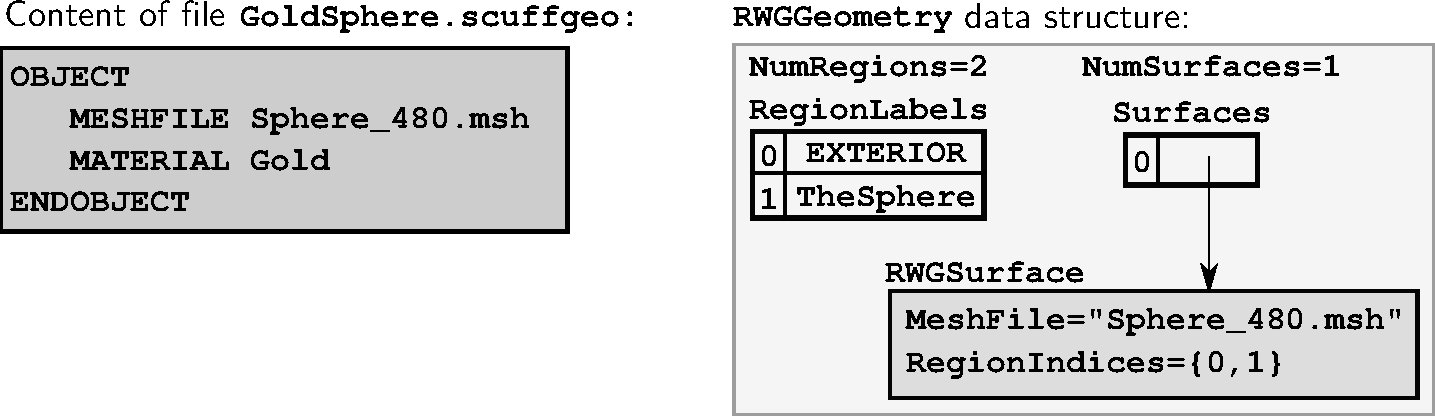
\includegraphics{RWGGeometryDataFields1.pdf}}
\caption{A simple \texttt{.scuffgeo} file and some fields in the 
         corresponding \texttt{RWGGeometry} structure.}
\end{center}
\end{figure}
%####################################################################%

In the language of regions and surfaces discussed above,
each \texttt{OBJECT} statement adds one new region and 
one new surface to a geometry. The newly added region 
is always taken to be the interior region associated
with the newly added surface, and corresponds to the
volume inside the object; the new surface exists at 
the interface between this region and the exterior
medium.

We said above that surface meshes for compact objects 
should be \textit{closed} surfaces. The exception to 
this statement is that PEC (perfectly electrically
conducting) or IPEC (imperfectly electrically 
conducting) bodies may be described by open surfaces.
(An IPEC body is a PEC body with finite surface 
conductivity). For both PEC and IPEC bodies the
interior fields vanish identically, and there
is no need for such bodies to have finite
interior volume. An \texttt{OBJECT} statement 
declaring a new PEC or IPEC object adds one new surface
but \textit{not} one new region to the geometry.

\subsection*{Simple geometries: Nested objects} 

It is possible for an object defined by an
\texttt{OBJECT} declaration to be fully 
contained inside another \texttt{OBJECT}. 
The nesting inclusion relationship is automatically 
detected by \ls. 

\subsection*{More complicated geometries: \texttt{REGION}
             and \texttt{SURFACE} statements}

Some geometries are too complicated to be defined 
as collections of compact objects bounded by closed 
surfaces. One example is a composite sphere in which 
the upper and lower hemispheres consist of different 
materials. Another example is a metallic nanoparticle 
(say, a disc) lying atop a dielectric substrate. The 
common feature of these two examples that prevents 
description in terms of simple closed objects is the 
presence of \textit{multi-material junctions}; these
are one-dimensional subspaces at which three
or more material regions meet. 
For the composite sphere, the multi-material junction 
would be the equator; for the disc on the substrate, 
it would be the lower circumference of the disc.

Geometries like this are described in \lss
using \texttt{REGION} and \texttt{SURFACE}
statements. For example, the composite sphere
above may be specified like this:
%####################################################################%
\begin{figure}[H]
\begin{center}
\resizebox{\textwidth}{!}{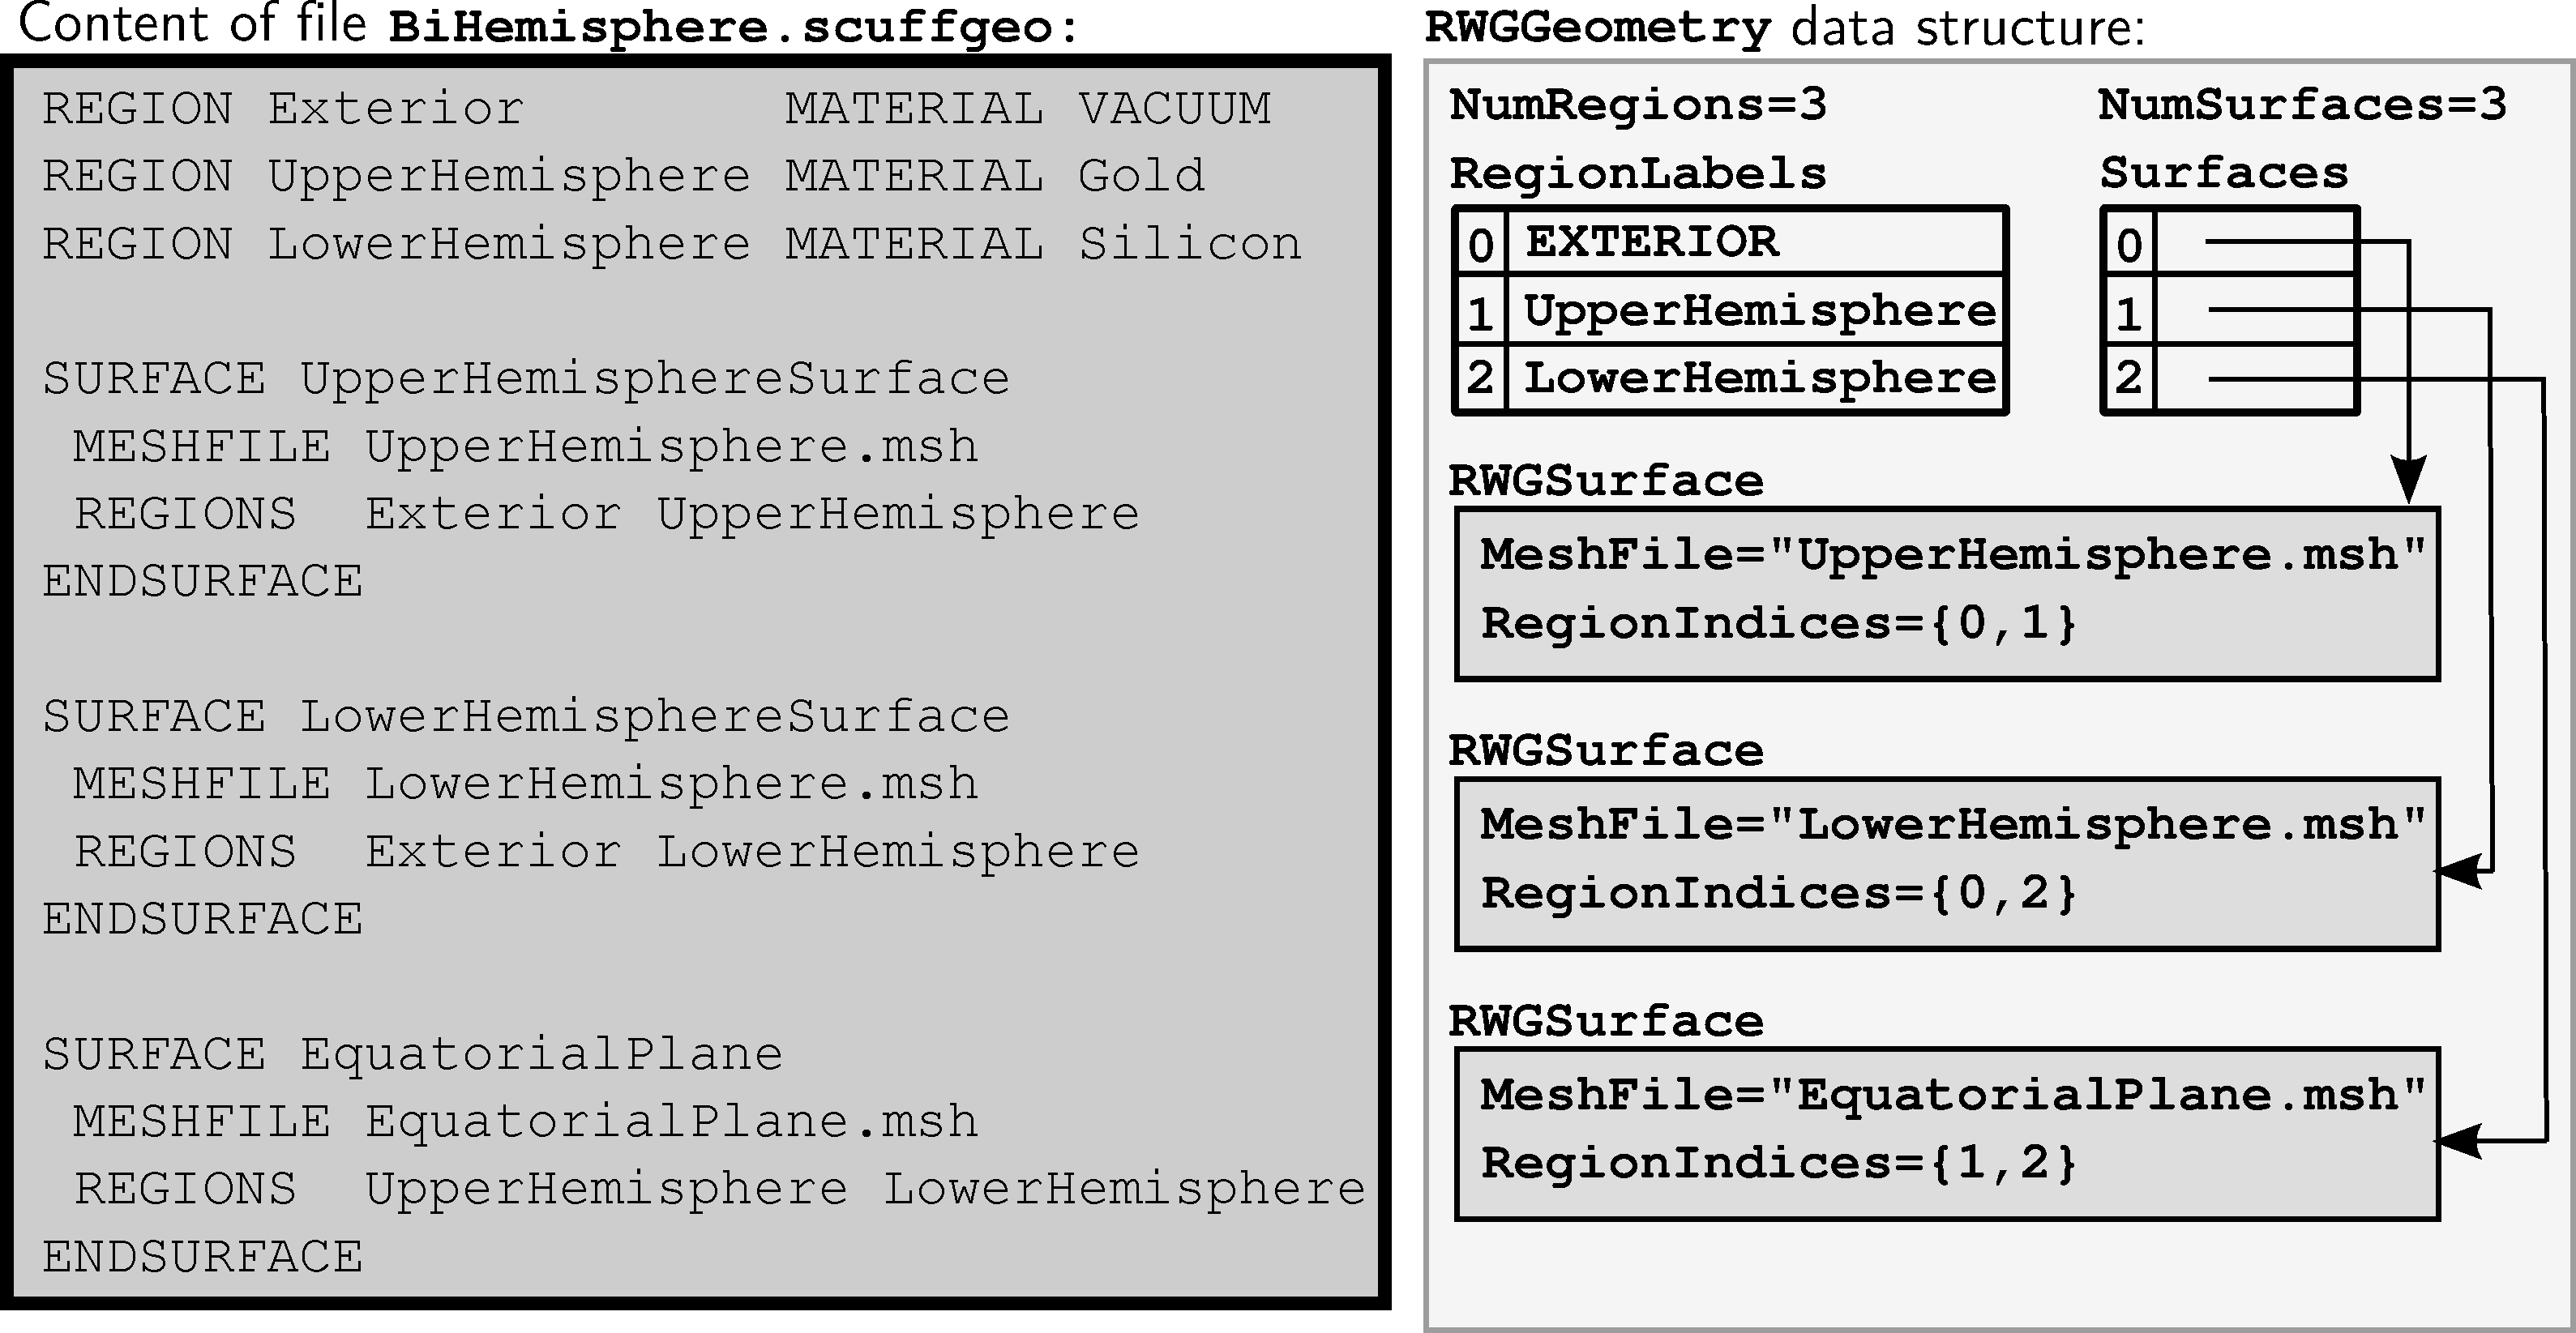
\includegraphics{RWGGeometryDataFields2.pdf}}
\caption{A more complex \texttt{.scuffgeo} file and some fields in the 
         corresponding \texttt{RWGGeometry} structure.}
\end{center}
\end{figure}
%####################################################################%
\subsection*{Extended geometries: \texttt{LATTICE}
             statements}

Extended geometries are described using \texttt{LATTICE}
statements in the \texttt{scuffgeo} file.
For example, here's an infinite square-lattice array 
of gold spheres:
%
\begin{verbatim}
LATTICE
        VECTOR 1 0 
        VECTOR 0 1 
ENDLATTICE

OBJECT TheSphere
        MESHFILE Sphere_480.msh
        MATERIAL Gold
ENDOBJECT
\end{verbatim}
%

It is also possible for surfaces to straddle 
the lattice-cell boundaries. This will be the 
case, for example, if you are describing an
infinite planar surface (possibly with
holes). In this case, the surface mesh must
be \textit{compatible} with the lattice specification,
in the sense that every triangle edge that 
lies on the unit-cell boundary must have an
image edge lying one lattice-translate away.

\subsection*{Extended geometries in which the exterior medium
             is non-contiguous}

In some extended geometries, it may be possible for the 
exterior medium to be non-contiguous. For example,
consider a thin film described by two planar surfaces  
(the upper and lower surfaces of the film) with a
\texttt{LATTICE} statement indicating the surfaces
are infinitely extended (comprised of an infinite
2D lattice of the unit-cell surfaces).
In this case, you probably think of the region above the 
upper surface and the region below the lower surface as 
both belonging to the same region, but as far as 
\lss is concerned they must be two different regions.

The reason for this is the following: Suppose both
the upper half-space and the lower half-space were
the same region (say \texttt{Exterior}). Then the upper 
and lower surfaces of the slab would both have 
\texttt{Exterior} as one of the two regions 
at whose interface they lie, and thus surface currents
on both the upper and lower surfaces would contribute 
to the scattered fields at all points in \texttt{Exterior}.
But this would be incorrect: Points in the upper half-space
receive scattered-field contributions only from currents
on the upper surface, while points in the lower half-space 
receive contributions only from the lower surface. 

The situation would be different if the upper and lower 
half-spaces were \textit{contiguous}---which would be
the case, for example, if the thin-film slab had a hole
in it. In this case, the upper and lower film surfaces
(as well as the hole sidewall surfaces) all form 
part of a single bounding surface separating the 
film interior from \texttt{Exterior}, and hence surface
currents on all of these surfaces contribute to the
scattered fields at points in \texttt{Exterior}.

%%%%%%%%%%%%%%%%%%%%%%%%%%%%%%%%%%%%%%%%%%%%%%%%%%%%%%%%%%%%%%%%%%%%%%
%%%%%%%%%%%%%%%%%%%%%%%%%%%%%%%%%%%%%%%%%%%%%%%%%%%%%%%%%%%%%%%%%%%%%%
%%%%%%%%%%%%%%%%%%%%%%%%%%%%%%%%%%%%%%%%%%%%%%%%%%%%%%%%%%%%%%%%%%%%%%
\newpage
\section{Representation of Surface Currents in \ls}

\subsection*{Surface Currents}

\lss is based on the surface-integral-equation approach
to computational electromagnetism. In this approach, the
fundamental unknowns are tangential \textit{surface
currents} flowing on the surfaces that lie at the 
interface between homogeneous material regions.

\subsubsection*{Electric and magnetic surface currents at dielectric 
                interfaces}
For the general case of a surface lying between two
dielectric regions, we have both an electric 
surface-current distribution $\vb K(\vb x)$ and a 
magnetic surface-current distribution $\vb N(\vb x)$
(here $\vb x$ is a point lying on the surface).
Both $\vb K$ and $\vb N$ are strictly \textit{tangential}
to the surface; they have no normal component.

\subsubsection*{Physical interpretation of surface currents}

One way to interpret the $\vb K$ and $\vb N$ currents
is as effective source distributions confined to the surfaces. 
In a real scattering problem involving dielectric bodies, the 
incident fields induce a physical volume electric current 
distribution $\vb J(\vb r)$ which is nonzero for all points 
$\vb r$ inside dielectric bodies, and the scattered fields 
are just the fields radiated by this source distribution.
The surface currents $\vb K$ and $\vb N$ are \textit{fictitious}
or (``effective'') source distributions with the property 
that the fields they radiate exactly reproduce the 
field radiated by the physical source distribution $\vb J$,
both inside and outside the body. What is unphysical about 
$\vb K$ and $\vb N$ is that \textbf{(a)} they are confined to 
the surfaces, whereas the physical induced source distribution
$\vb J$ exists throughout the volume, and \textbf{(b)} they
include magnetic currents $\vb N$, i.e. moving magnetic monopoles,
which do not actually exist in our universe.\footnote{Perhaps
we should say no more than \textit{one} of them exists in our 
universe: \url{http://prl.aps.org/abstract/PRL/v48/i20/p1378_1}.}
However, the fields radiated by $\vb K$ and $\vb N$ are 
perfectly physical.

Another, perhaps more direct, way to interpret the 
$\vb K$ and $\vb N$ currents is that they are nothing 
but rotated versions of the tangential components of 
the total electric and magnetic fields at the 
surface, i.e. we have 
$$ \vb K(\vb x) = \vbhat{n}\times \vb H\sups{tot}(\vb x), 
   \qquad 
   \vb N(\vb x) =-\vbhat{n}\times \vb E\sups{tot}(\vb x).
$$

\subsubsection*{Electric surface currents on PEC surfaces}

In the special case of a PEC surface---whether closed or
open---the magnetic surface current vanishes identically
($\vb N=0$) and only the electric surface current 
$\vb K$ is nonzero. In this case, the two interpretations of the 
surface currents discussed above coincide physically: 
Incident fields really do excite physical electric
currents on the surfaces of PEC bodies, these currents
really are strictly confined to the surfaces (in the
idealized limit of a \textit{perfect} electric conductor),
and the field radiated by these induced currents
really is the full scattered field.

\subsection*{RWG Basis Functions}
%####################################################################%
\begin{figure}
\begin{center}
\resizebox{\textwidth}{!}{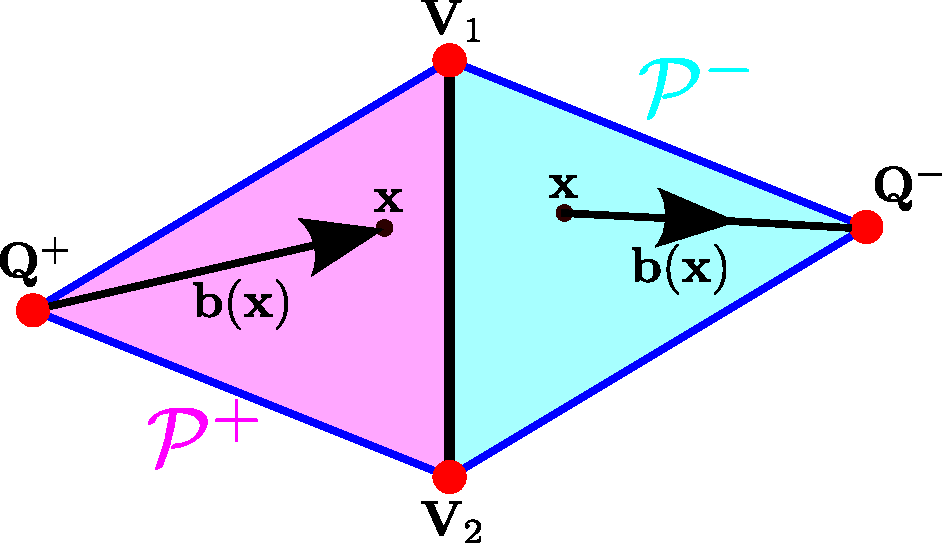
\includegraphics{RWGBasisFunctionNotation.pdf}}
\caption{Notation for RWG basis functions.}
\label{RWGNotationFigure}
\end{center}
\end{figure}
%####################################################################%

\lss uses RWG basis functions\footnote{S. M. Rao, D. R. Wilton, 
A. W. Glisson, \textit{IEEE Trans.\ Antennas Propagat.} 
\textbf{AP-30} 409 (1982).} to describe electric and magnetic 
surface currents flowing on the surfaces in a geometry. 
Each RWG basis function is assigned to a single interior
edge in a surface mesh discretization, and is nonvanishing
only on the two triangular panels that share that 
edge. 

To construct the RWG basis function associated with an 
edge (Figure \ref{RWGNotationFigure}), arbitrarily choose one 
of the two panels to be the \textit{positive} panel $\mc P^+$ 
associated with the basis function, while the other panel is the 
\textit{negative} panel $\mc P^-$. Let the vertices of the 
common edge be $\vb V_1$ and $\vb V_2$, and let the third vertex of 
$\mc P^+$ be the positive or \textit{source} vertex 
$\vb Q^+$ for the basis function, 
while the other opposite vertex will be the 
negative or \textit{sink} vertex $\vb Q^-$. Then 
the RWG basis function $\vb b(\vb x)$ associated with the
edge is defined as follows:
$$ \vb b(\vb x) = 
   \begin{cases}   
  +\frac{l}{2A^+}(\vb x - \vb Q^+), \qquad &\vb x \in \mc P^+ \\ 
  -\frac{l}{2A^+}(\vb x - \vb Q^-), \qquad &\vb x \in \mc P^- \\ 
   0, \qquad &\text{otherwise}
   \end{cases}
$$
where $l$ is the length of the common edge (the distance
$\vb V_1 \vb V_2$) and $\vb A^\pm$ are the areas of $\mc P^\pm$.
Thus the RWG function describes a current that emanates 
from $\vb Q^+$, grows linearly in strength as it flows along
the surface of $\mc P^+$ toward the common edge, begins
decreasing linearly in strength after crossing over that
edge into $\mc P^-$, and is sunk into $\vb Q^-$. There
is no current flow outside the pair of panels because
$\vb b(\vb x)$ has no component normal to any of the 
four exterior edges of the panel pair.

Figure \ref{RWGBasisFunctionFigure} illustrates some of the 
\lss data structures associated with a single RWG basis function
embedded in a surface mesh.
%####################################################################%
\begin{figure}
\begin{center}
\resizebox{\textwidth}{!}{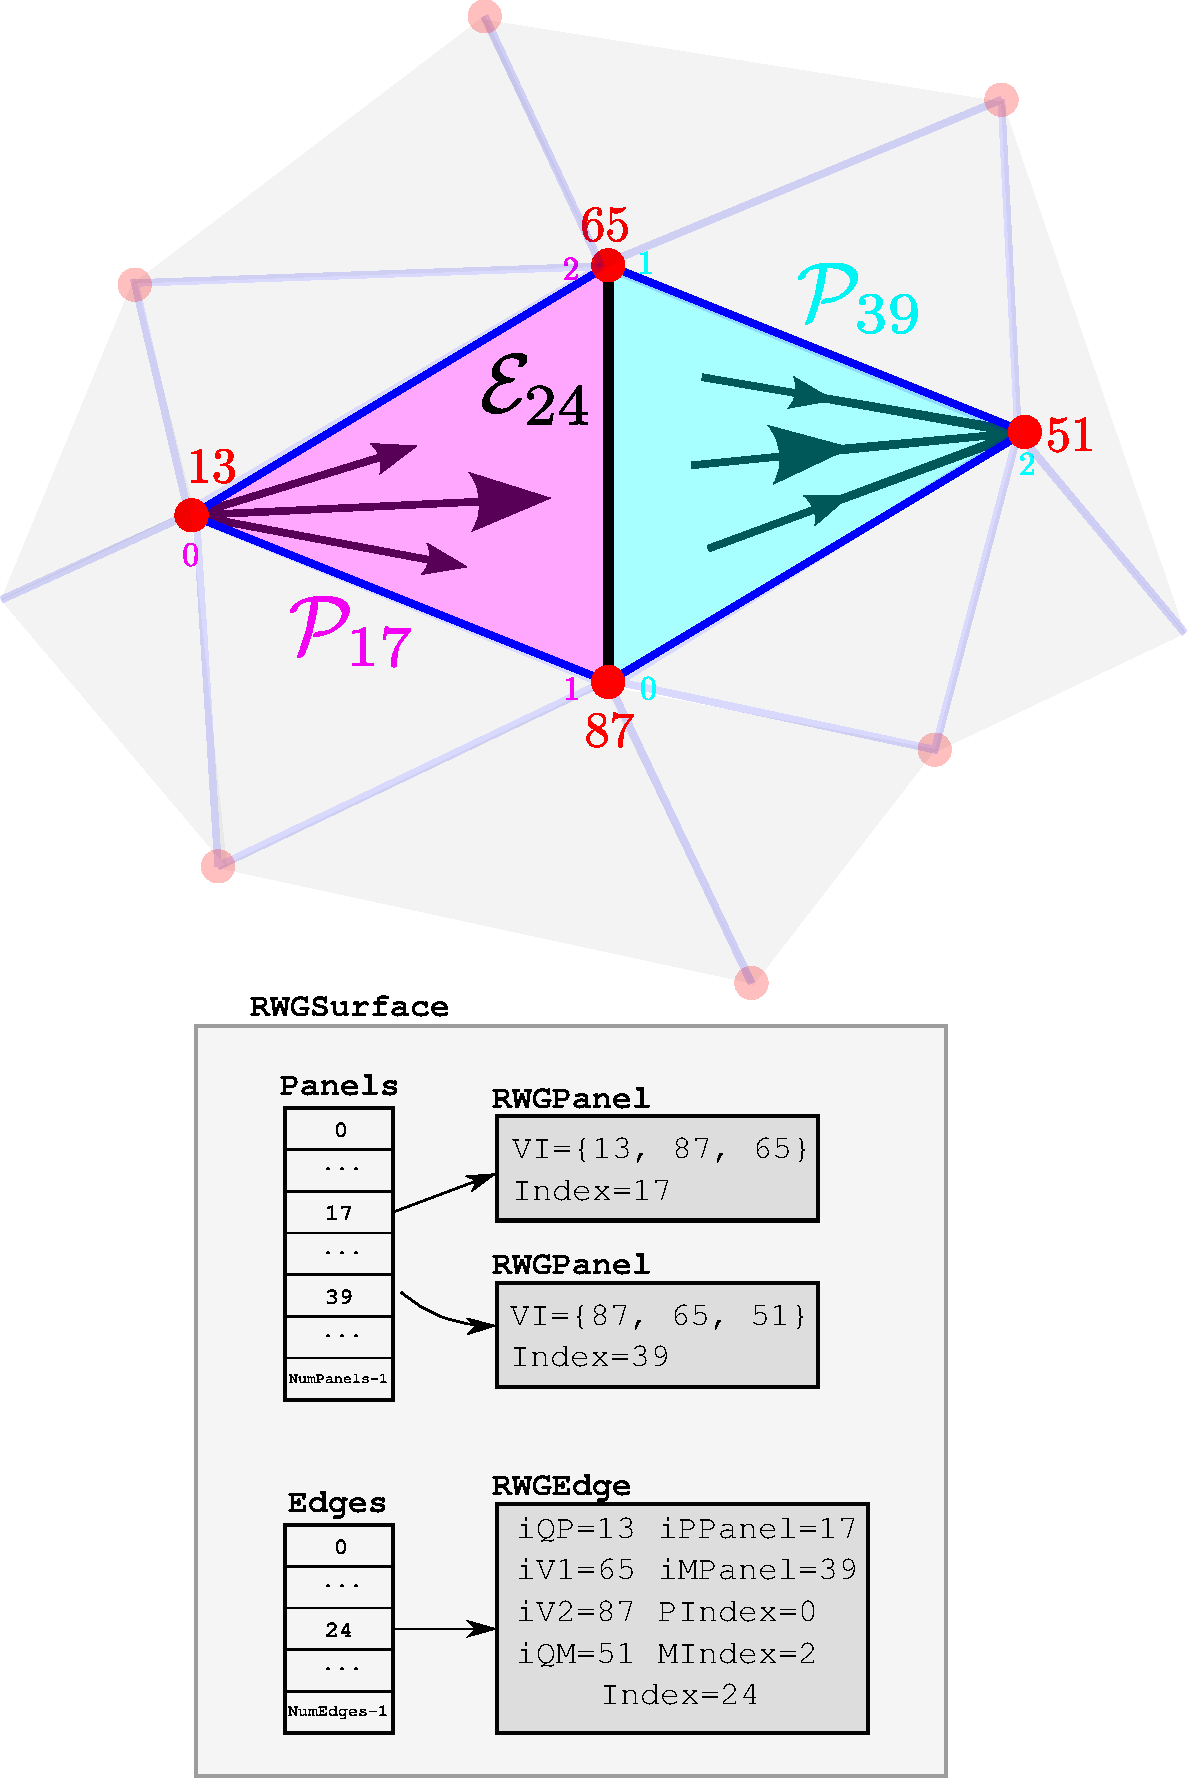
\includegraphics{RWGBasisFunction.pdf}}
\caption{A single RWG basis function associated with an internal edge 
         on an \texttt{RWGSurface}, and some portions of data structures 
         within the corresponding \texttt{RWGSurface} instance that 
         describe this basis function.}
\label{RWGBasisFunctionFigure}
\end{center}
\end{figure}
%####################################################################%

\subsection*{Half-RWG Basis Functions}

It is also possible to assign basis functions to 
\textit{exterior} edges of surface meshes, i.e.
edges that lie on the boundary of open surfaces.
In contrast to interior edges, exterior edges 
are associated within only one panel, not two
panels. {\sc scuff-em} adopts the convention
that this panel is the positive panel $\mc P^+$
for the edge, while there is no negative panel
$\mc P^-$. For exterior edges, the \texttt{iMPanel}
field of the \texttt{RWGEdge} structure 
is set to \texttt{-1}.


